\section{Controllers Implementation}
The implementation of the controllers can not be done having them as a continuous expression due to the discrete operation of the microcontroller. 

In order to discretize the controllers in the system, they need to be expressed in terms of the $z$ operator, the equivalent to the Laplace operator in the discrete domain. This transformation is done through the Tustin (bilinear) approximation in which the $s$ term in the transfer function is substituted as seen in \autoref{tustin}. \fxnote{Source Feedback control of dynamic systems}
\begin{flalign}
	s\approx\frac{2}{T}\frac{z-1}{z+1}
	\label{tustin}
\end{flalign}
\begin{where}
	\va{s}{is the Laplace Operator}{}
	\va{z}{is the discrete operator}{}
	\va{T}{is the sampling time}{}
\end{where}
The Tustin approximation maps the Laplace stable region into the discrete stable region, that is, the unit circle, as seen in \autoref{fig:tustinmap}, for these reason, is one of the most used discretization methods.
\begin{figure}[H]
	\includegraphics[scale=.7]{figures/tustinmapping}
	\centering			
	\captionof{figure}{Attitude control loop Bode diagram.} 
	\label{fig:tustinmap}
\end{figure} 
The discrete transfer function is then transformed into a difference equation to obtain the expression to be applied in the microcontroller. This is done taking into account that a $z^{-1}$ term implies taking the previous sample of the data. 

When discretizing the controller, the sampling time must also be considered. In the system at hand, the sampling frequency is limited by the sensor data (Vicon System) to be 100 Hz as a maximum. The lower limit comes from the bandwidth of the controllers as for the discretization not to affect the controller response, the sampling frequency should be 25 times higher than the bandwidth of the control loop \fxnote{SOURCE}. The fastest control loop in the system is the attitude controller and has a bandwidth of 5 rad/s, that is, 0.8 Hz. This implies a minimum sampling frequency of 20 Hz.\fxnote{CHECK NUMBERS}

The chosen sampling frequency in the system is 30 Hz in order to keep the controllers with a good performance an far from the 100 Hz that Vicon provides in order to have time for processing the communication task and the control program.\fxnote{CHECK NUMBERS}
\subsection{Attitude Controllers}
The attitude controller is mainly composed of gains formed by the state feedback, the integral and the observer matrices. this makes the discretization easier as there are no $s$ terms in the controller. There are though two integrators, one is in the observer and the other one is placed in the integral term of the controller.

The discrete form of an integrator using the bilinear approximation is shown in \autoref{discreteIntegrator}. The formula shows how the integrator in the integral term of the attitude control looks like when discretized.  
\begin{flalign}
	\frac{x_{int}}{\phi_{ref}-\phi}=\frac{x_{int}}{e_{\phi}} \approx \frac{T}{2}\frac{z+1}{z-1}
	\label{discreteIntegrator}
\end{flalign}
This transformation yields a difference equation as seen in \autoref{discreteIntegratordifferences}, which shows the example in the roll angle case. It gives the current value of the integral state as a function of the previous integral state and the current and the previous error between the angular reference and the angular data.
\begin{flalign}
	x_{int}(k)=x_{int}(k-1) + \frac{T}{2} e_{\phi}(k) + \frac{T}{2} e_{\phi}(k-1)
	\label{discreteIntegratordifferences}
\end{flalign}

The effect of the discretization in the designed attitude controllers is shown in \fxnote{INCLUDE COMPARISON}. As the attitude information is transmitted through the network, the delay effect and packet loss are also included in the discrete simulation by using the network simulator TrueTime. 

It can be seen that the performance of the discrete attitude controller is still able to track the given references with a similar response. 
\subsection{Translational Controllers}
The translational controllers are all proportional controllers except the velocity z controller, which is a PI controller. The gains are the same in both continuous and discrete domains but the PI needs to be discretized with the Tustin rule. 

The discrete version of the z controller is shown in \autoref{discreteVelocityZcontroller}.
\begin{flalign}
	\frac{\omega_{sum}}{e_{\dot{z}}} = tf_{cont} \approx tf_discrete
	\label{discreteVelocityZcontroller}
\end{flalign}

From the above equation, the difference equation that should be implemented in the microcontroller is calculated. The final equation is shown in \autoref{discreteVelocityZcontrollerdiferences}. \fxnote{CHECK NUMBERS IN THE EQUATIONS}

\begin{flalign}
	\omega_{sum}(k)= \omega_{sum}(k-1) + e_{\dot{z}}(k) + e_{\dot{z}}(k-1)
	\label{discreteVelocityZcontrollerdiferences}
\end{flalign}

In \fxnote{INCLUDE COMPARIONS OF THE X Y AND Z} the comparison of the translational controllers discrete and continuous versions. In the simulation, the delay and the package loss network effects are also included, as not only the sampling rate affects the response but also these two network effects. 


It can be seen that the response bla bla bla